\documentclass[a4paper]{article}
\usepackage[pdftex]{graphicx}
\usepackage[utf8]{inputenc}
\usepackage{enumerate}
\usepackage{siunitx}
\sisetup{locale=DE}
\usepackage{icomma}
\usepackage{colortbl}
\usepackage{multirow}
\usepackage{amssymb}
\usepackage{tikz}
\usetikzlibrary{positioning}
\usepackage{href-ul}
\hypersetup{
	colorlinks=true,
	linkcolor=blue,
	urlcolor=blue}
\usepackage{geometry}
\geometry{a4paper, top=15mm, left=15mm, right=15mm, bottom=15mm,
	headsep=10mm, footskip=12mm}


\begin{document}
	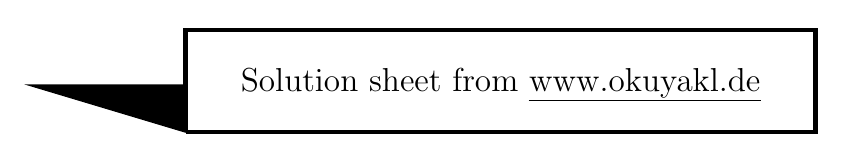
\begin{tikzpicture}(10,3)
		\draw[ultra thick](2,0) --(10,0) -- (10,1.3) --(2,1.3) -- (2,0); 
		\draw[fill=black](2,0)-- (0,.6) -- (2,.6) -- (2,0); 
		\node at (6,.6) {\large Solution sheet from \href{https://www.okuyakl.de}{www.okuyakl.de}};
	\end{tikzpicture}
	\vspace{0.5 cm}
	
	%Title
	{\bf Parallel and Series Connection of Resistors}.\\
	\begin{enumerate}[1.]

{\bf \item The individual resistors have the following values:}\\

\renewcommand{\arraystretch}{2}
\begin{tabular}{|>{\columncolor[gray]{.8}}p{1.5 cm}|p{1.5 cm}|p{1.5 cm}|p{1.5 cm}|}
	\hline
	\rowcolor[gray]{.8}	 $R$ & $U$ & $I$	& $P$	\\
	\hline
	$\SI{10}{\ohm}$	& $\SI{5}{\volt}$	& $\SI{0.5}{\ampere}$&$\SI{2.5}{\watt}$ \\
	\hline
	$\SI{33}{\ohm}$& $\SI{5}{\volt}$& $\SI{0.15}{\ampere}$& $\SI{0.76}{\watt}$\\
	\hline
	$\SI{100}{\ohm}$& $\SI{5}{\volt}$& $\SI{0.05}{\ampere}$& $\SI{0.25}{\watt}$\\
	\hline
\end{tabular}\\

{\bf The calculated resistance values:}\\

\begin{minipage}{0.5\textwidth}
	\item Series connection
	
	\renewcommand{\arraystretch}{2}
	\begin{tabular}{|>{\columncolor[gray]{.8}}p{1.5 cm}|p{1.5 cm}|p{1.5 cm}|p{1.5 cm}|}
		\hline
		\rowcolor[gray]{.8}	 $R_1 +R_2$  & $\SI{10}{\ohm}$	& $\SI{33}{\ohm}$	& $\SI{100}{\ohm}$	\\
		\hline
		$\SI{10}{\ohm}$	& $\SI{20}{\ohm}$	&  $\SI{43}{\ohm}$	&  $\SI{110}{\ohm}$	\\
		\hline
		$\SI{33}{\ohm}$	&  $\SI{43}{\ohm}$	&  $\SI{66}{\ohm}$	& $\SI{133}{\ohm}$	\\
		\hline
		$\SI{100}{\ohm}$	& $\SI{110}{\ohm}$	 &  $\SI{133}{\ohm}$	&  $\SI{200}{\ohm}$	\\
		\hline
	\end{tabular}
\end{minipage}
\hfill
\begin{minipage}{0.5\textwidth}
	\item Parallel connection
	
	\renewcommand{\arraystretch}{2}
	\begin{tabular}{|>{\columncolor[gray]{.8}}p{2 cm}|p{1.5 cm}|p{1.5 cm}|p{1.5 cm}|}
		\hline
		\rowcolor[gray]{.8}	 $\left(\frac{1}{R_1}+\frac{1}{R_2}\right)^{-1}$ & $\SI{10}{\ohm}$	& $\SI{33}{\ohm}$	& $\SI{100}{\ohm}$	\\
		\hline
		$\SI{10}{\ohm}$	&  $\SI{5}{\ohm}$	&  $\SI{7.7}{\ohm}$	&  $\SI{9.1}{\ohm}$	\\
		\hline
		$\SI{33}{\ohm}$	&  $\SI{7.7}{\ohm}$	&  $\SI{17}{\ohm}$	&  $\SI{25}{\ohm}$	\\
		\hline
		$\SI{100}{\ohm}$	& $\SI{9.1}{\ohm}$	 &  $\SI{25}{\ohm}$	&  $\SI{50}{\ohm}$	\\
		\hline
	\end{tabular}
\end{minipage}
{\bf \item Which resistors do you connect to obtain the ...}\\

\begin{enumerate}[a)]
	
	\hspace{-2 cm}
	\begin{minipage}{0.3\textwidth}
		\includegraphics[width=5 cm]{1wisch243.pdf}
	\end{minipage}
	\hspace{-0.5cm}
	\begin{minipage}{0.3\textwidth}
		\item ...largest possible total resistance?\\
		
		\renewcommand{\arraystretch}{2} \begin{tabular}{|>{\columncolor[gray]{.8}}p{1cm}|p{0.8cm}|p{0.8cm}|p{0.8cm}|p{0.9cm}|}
			\hline
			\rowcolor[gray]{.8}	  & $R$ & $U$	& $I$	 & $P$\\
			\hline
			1 & $\SI{100}{\ohm}$& $\SI{4,0}{\volt}$& $\SI{40}{\milli\ampere}$&$\SI{0,16}{\watt}$ \\
			\hline
			2	&  $\SI{100}{\ohm}$& $\SI{1,0}{\volt}$& $\SI{10}{\milli\ampere}$&$\SI{10}{\milli\watt}$ \\
			\hline
			3 &  $\SI{33}{\ohm}$& $\SI{1,0}{\volt}$& $\SI{30}{\milli\ampere}$&$\SI{30}{\milli\watt}$  \\
			\hline
			Total &  $\SI{125}{\ohm}$& $\SI{5,0}{\volt}$& $\SI{40}{\milli\ampere}$&$\SI{0,2}{\watt}$  \\
			\hline
		\end{tabular}
	\end{minipage}
	\hspace{1cm}
	\begin{minipage}{0.3\textwidth}
		\item ...the smallest total resistance?
		
		\renewcommand{\arraystretch}{2}
		\begin{tabular}{|>{\columncolor[gray]{.8}}p{1cm}|p{0.8cm}|p{0.8cm}|p{0.8cm}|p{0.9cm}|}
			\hline
			\rowcolor[gray]{.8}	  & $R$ & $U$	& $I$	 & $P$ \\
			\hline
			1 &  $\SI{10}{\ohm}$& $\SI{2,8}{\volt}$&  $\SI{0,28}{\ampere}$&$\SI{0,78}{\watt}$ \\
			\hline
			2	& $\SI{10}{\ohm}$ & $\SI{2,2}{\volt}$& $\SI{0.22}{\ampere}$&$\SI{0.48}{\watt}$  \\
			\hline
			3 &  $\SI{33}{\ohm}$& $\SI{2.2}{\volt}$&  $\SI{66}{\milli\ampere}$&$\SI{0.15}{\watt}$  \\
			\hline
			Total & $\SI{18}{\ohm}$ & $\SI{5.0}{\volt}$&  $\SI{0.28}{\ampere}$&$\SI{1.4}{\watt}$ \\
			\hline
		\end{tabular}
	\end{minipage}
	
	\hspace{-2 cm}
	\begin{minipage}{0.3\textwidth}
		\includegraphics[width=5 cm]{2wisch243.pdf}
	\end{minipage}
	\hspace{-0.5cm}
	\begin{minipage}{0.3\textwidth}
		\item ...the largest total resistance?
		\renewcommand{\arraystretch}{2}
		\begin{tabular}{|>{\columncolor[gray]{.8}}p{1cm}|p{0.8cm}|p{0.8cm}|p{0.8cm}|p{0.9cm}|}
			\hline
			\rowcolor[gray]{.8}	  & $R$ & $U$	& $I$	 & $P$ \\
			\hline
			1 &  $\SI{100}{\ohm}$& $\SI{5.0}{\volt}$&  $\SI{50}{\milli\ampere}$&$\SI{0.25}{\watt}$  \\
			\hline
			2	& $\SI{100}{\ohm}$ & $\SI{3.8}{\volt}$&  $\SI{38}{\milli\ampere}$&$\SI{0.14}{\watt}$  \\
			\hline
			3 & $\SI{33}{\ohm}$ & $\SI{1.2}{\volt}$&  $\SI{38}{\milli\ampere}$&$\SI{50}{\milli\watt}$ \\
			\hline
			Total &  $\SI{57}{\ohm}$& $\SI{5.0}{\volt}$&  $\SI{88}{\milli\ampere}$&$\SI{0.44}{\watt}$ \\
			\hline
		\end{tabular}
		\end{minipage}
		\hspace{1cm}
		\begin{minipage}{0.3\textwidth}
		\item ...to obtain a low total resistance?
		
		\renewcommand{\arraystretch}{2}
		\begin{tabular}{|>{\columncolor[gray]{.8}}p{1cm}|p{0.8cm}|p{0.8cm}|p{0.8cm}|p{0.9cm}|}
			\hline
			\rowcolor[gray]{.8}	  & $R$ & $U$	& $I$	 & $P$\\
			\hline
			1 &  $\SI{10}{\ohm}$&$\SI{5.0}{\volt}$ & $\SI{0.5}{\ampere}$&$\SI{2.5}{\watt}$  \\
			\hline
			2	& $\SI{10}{\ohm}$ & $\SI{1.2}{\volt}$& $\SI{0.12}{\ampere}$&$\SI{0.13}{\watt}$  \\
			\hline
			3 &  $\SI{33}{\ohm}$& $\SI{3.8}{\volt}$&  $\SI{0.12}{\ampere}$&$\SI{0.44}{\watt}$  \\
			\hline
			Total &  $\SI{8.1}{\ohm}$& $\SI{5.0}{\volt}$&  $\SI{0.62}{\ampere}$&$\SI{3.1}{\watt}$ \\
			\hline
		\end{tabular}
		\end{minipage}
		
		
	\end{enumerate}


\end{enumerate}

\begin{center}
\includegraphics[width=7 cm]{../../viecher/eendcomic.pdf}

Click here to return to the \href{https://www.okuyakl.de/phys/p8wipareiL243/ae243.pdf}{worksheet}
\end{center}

\end{document}